%NOTES
%Turing machines have to work on empty word aswell
% We need at least 3 tapes according to lib version, we can change that if we want.
% Source - https://tex.stackexchange.com/a/219399
% Posted by egreg, modified by community. See post 'Timeline' for change history
% Retrieved 2026-11-10, License - CC BY-SA 3.0


\documentclass[UTF8]{article}
\usepackage{amsmath}
\usepackage{amssymb}
\usepackage{mathtools}
\usepackage{graphicx}
\usepackage{epstopdf}
\usepackage{inputenc}
\usepackage{geometry}
\geometry{left=2.5cm,right=2.5cm,top=2.5cm,bottom=2.5cm}
\usepackage{hyperref}
\usepackage{amsfonts}
\usepackage{cleveref} 
\usepackage{tikz}
\usepackage{graphicx}
\usetikzlibrary{positioning}

% custom commands
\renewcommand{\L}{{L_{\tiny{AM}}}}
\newcommand{\Z}{\mathbb{Z}}
\newcommand{\R}{\mathbb{R}}
\newcommand{\set}[1]{\{#1\}}

\begin{document}

\title{
  A Unary Non-Regular Language in $O(\log \log n)$ Space \\
    \large
        Formalizing Analysis of Algorithms \\
        Project Proposal}

\author{Jora Zeneli, Laura Kribben, Lasse Reith, Elia Riva}

\date{13 November 2026}

\maketitle

\tableofcontents

\newpage

\section{Motivation}
% IDEA: Motivate why the paper was written and present its results
Iwama~\cite{iwamaregular} showed that every language that is decidable in $o(\log \log n)$ space is regular.
Thus, the optimal upper bound space complexity for deciding a non regular language is $O(\log \log n)$ 
% Thus, for every non regular language, an algorithm deciding it requires a minimum space complexity of $O(\log \log n)$.
Alt and Mehlhorn~\cite{Lang-OneSymbAlph-LogLogn-HM-1975} present a unary non regular language $L$ that is decidable in $O(\log \log n)$ space. 
This project aims at formalizing the papers proof in Lean~4~\cite{lean4}, by constructing a turing machine that decides $L$ and takes the proposed space.

According to the paper, $L_{AM}$ is the language that consists of all words $a^n$ such that the smallest integer that does not divide n is a power of two.
We define $L_{AM}$ in terms of the helper function $q(n)$ with $n \geq 1$:
$$ {q(n) := \min\{ k\in\mathbb N^+ \mid k\nmid n\}}, \qquad \qquad  \L := \{a^n \mid \exists\ i \in \mathbb N : q(n) = 2^i  \}.$$
To decide $\L$ the paper uses the following algorithm: \\
Input: 
$q \leftarrow 1$
Repeat: 
$q \leftarrow q + 1; \quad p \leftarrow n \mod q \text{ until } p \neq 0$.
If q is a power of two, accept, else reject. 
The space complexity of the algorithm follows from the lemma $\exists c>0:\; q(n) \leq c \cdot \log n$, which is also shown in the paper.

\section{Modeling} 
In this section, we give a general description on how we plan to formalize Turing machines in Lean, which we later use to model the algorithm proposed by Alt and Mehlhorn~\cite{Lang-OneSymbAlph-LogLogn-HM-1975}.

\subsection{Turing Machines (TMs)}

A Turing machine is an abstract model in computer science to reason about computation. 
It consist of a finite control automaton and one or multiple tapes which it can read and write on.
Based on the current control state and symbols under heads, the machine decides where to move each head next, what to write in their tapes, to which control state to 2 to and when to halt computation.
CSLib already provides a formalization of deterministic multi-tape Turing machines. 
Depending on the suitability to our project, we either instantiate a machine using this existing formalization or adapt it to our needs. 
Our Turing machine will use one read-only input tape and one work tape. 
To measure the space complexity the CSLib provides the \texttt{spaceUsed} function that returns the number of tiles of the working tape that were visited. 


\subsection{Component TMs}
To facilitate the formalization of the algorithm, we break it down into simpler functions and languages, which we model as Turing machines.
We call them components; see \Cref{tab:compTMs}. 
% Each component TM either implements a function and stores its result on the work tape or tests a predicate. 
% To simplify the later composition, 
For compatibility reasons, all component TMs use the same tape architecture as the final machine: one read-only input tape and one work tape.
% We write $\operatorname{bin}(q)$ for the chosen binary representation of $q$ on the work tape.


\begin{table}[h]
    \centering
    \begin{tabular}{l|l|l|c}
        Name  & Purpose & Function & Language \\
        \hline
        $M_{\operatorname{succ}}$ & Increment $q$ & ${\operatorname{succ}}(q)\coloneqq q+1$ & $\set{0,1}^*$ \\

        $M_{\operatorname{divides}}$ &Test whether $q\mid n$ & ${\operatorname{mod}}(q)\coloneqq q$ & $\set{q \in \set{0,1}^* \mid n \operatorname{mod} q = 0}$ \\ 
           
        $M_{\operatorname{pow2}}$ &Test whether $q$ is a power of two &  ${\operatorname{pow2}}(q) \coloneq q$ & $\set{q \in \set{0,1}^* \mid \exists\ i \in \mathbb{N}.\; 2^i = q}$
        
    \end{tabular}
    \caption{Overview over the component TMs. The word $a^n$ is on the read-only tape and $q$ is on the working tape. The type of each function is $\set{0,1}^*\rightarrow \set{0,1}^*$.}
    \label{tab:compTMs}
\end{table}

\subsection{Composition of TM for deciding $\L$}
% describes how we plan to build models into
% We use the component TMs to construct $M_{\L}$, the Turing machine that decides $\L$.
% By combining the control automatons of the component TMs we can create a machine that calls the "subcomponent logic controls", which then either write on a part of the working tape or route to other logic parts. So we start with a working tape that has an imaginary split in the center. The LSBs of q and p are at that center and then expand outwards. 
% The first called component part in succ that increments q by one, this control part then call Mod which writes n mod q on the right side of the tape. We then call zero which calls succ iff p (right side) is != 0 and else calls pow2. pow2 then halts in an accepting state if q is a power of two. Else it halts and rejects.


We construct $M_{\L}$, the Turing machine deciding $\L$,
by combining the control states of the component TMs.
Roughly, we will model the composition by connecting exit states of each component to the entry states of the next component,
so that the components act as subprograms operating on
a shared read-only tape and work tape (see \Cref{fig:machines}).
The read-only tape contains the input word $a^n$.
The work tape contains $q$, which is initially is set to $1$.
The machine enters $\operatorname{succ}$, which increments $q$.
Next, the component TM $\operatorname{divides}$ tests whether $n \operatorname{mod}q=0$. If so, control returns to $\operatorname{succ}$; otherwise, it passes to $\operatorname{pow2}$.
The machine then accepts if $q$ is a power
of two and rejects otherwise. 
Each component leaves
the tape heads at positions required by the next component.
The read-only tape is never modified.

\begin{figure}[ht]
  \centering
  %\resizebox{0.7\textwidth}{!}{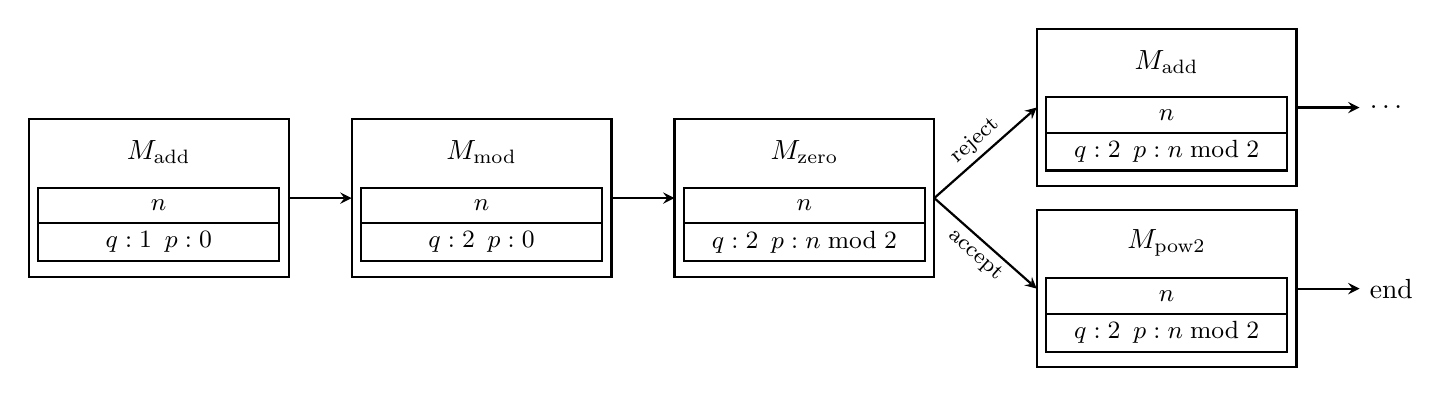
\begin{tikzpicture}[x=1cm, y=1cm, line width=0.8pt,
                    lbl/.style={font=\footnotesize, inner sep=2pt}]
  % ---- layout parameters (cm) ----------------------------------------
  \def\mw{3.3}     % width of one machine box
  \def\mh{2.0}     % height of one machine box
  \def\gap{0.8}    % horizontal gap between machines in the row
  \def\fork{1.3}   % horizontal gap before the stacked pair
  \def\vgap{0.3}   % vertical gap between the two stacked machines

  % #1 = title, #2 = counters
  \tikzset{
    pics/machine/.style 2 args={code={
      % outer box (lower-left corner at the pic's position)
      \draw (0,0) rectangle (\mw,\mh);
      \coordinate (-W) at (0,\mh/2);      % midpoint of left edge
      \coordinate (-E) at (\mw,\mh/2);    % midpoint of right edge
      % title
      \node at (\mw/2,1.58) {#1};
      % stacked boxes: n on top, counters below, sharing one border
      \draw (0.12,0.2) rectangle (\mw-0.12,1.13);
      \draw (0.12,0.68) -- (\mw-0.12,0.68);
      \node at (\mw/2,0.905) {\small $n$};
      \node at (\mw/2,0.44) {\small #2};
    }}
  }
  % row of three machines
  \pic (m1) at (0,0)                {machine={$M_{\text{add}}$}{$q : 1 \enspace p : 0$}};
  \pic (m2) at ({1*(\mw+\gap)},0)   {machine={$M_{\text{mod}}$}{$q : 2 \enspace p : 0$}};
  \pic (m3) at ({2*(\mw+\gap)},0)   {machine={$M_{\text{zero}}$}{$q : 2 \enspace p : n \bmod 2$}};

  % column of two machines, centred vertically on the row
  \pic (m4) at ({3*\mw+2*\gap+\fork},{(\mh+\vgap)/2})   {machine={$M_{\text{add}}$}{$q : 2 \enspace p : n \bmod 2$}};   % top
  \pic (m5) at ({3*\mw+2*\gap+\fork},{-(\mh+\vgap)/2})  {machine={$M_{\text{pow2}}$}{$q : 2 \enspace p : n \bmod 2$}};  % bottom

  \node[anchor=west] (next) at ([xshift=\gap cm]m4-E) {\dots};
  \node[anchor=west] (end) at ([xshift=\gap cm]m5-E) {end};

  % arrows
  \draw[-stealth] (m1-E) -- (m2-W);
  \draw[-stealth] (m2-E) -- (m3-W);
  \draw[-stealth] (m3-E) -- node[lbl, above, sloped] {reject} (m4-W);
  \draw[-stealth] (m3-E) -- node[lbl, below, sloped] {accept} (m5-W);
  \draw[-stealth] (m4-E) -- (next);
  \draw[-stealth] (m5-E) -- (end);
\end{tikzpicture}}
  \resizebox{0.7\textwidth}{!}{

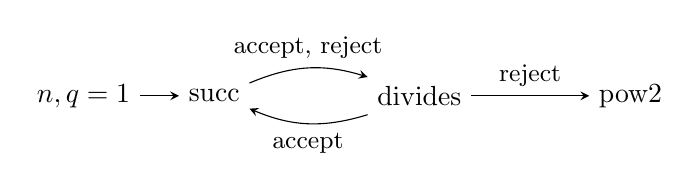
\begin{tikzpicture}[node distance=1.5cm, >=stealth,
                    lbl/.style={font=\small}]
  \node (start)                            {$n,q=1$};
  \node (succ)    [right=0.5cm of start]   {$\mathrm{succ}$};
  \node (divides) [right=of succ]          {$\mathrm{divides}$};
  \node (pow2)    [right=of divides]       {$\mathrm{pow2}$};

  \draw[->] (start) -- (succ);
  \draw[->] (succ)    to[bend left=20] node[lbl, above] {accept, reject} (divides);
  \draw[->] (divides) to[bend left=20] node[lbl, below]               {accept}           (succ);
  \draw[->] (divides) -- node[lbl, above] {reject} (pow2);
\end{tikzpicture}
}
  \caption{Composition of the machines.}
  \label{fig:machines}
\end{figure}


% We use the algorithm discussed in the paper. 
% For the first part, which is to determine the smallest number that does not divide the input, we use the component TMs $M_{\operatorname{zero}}$, $M_{\operatorname{succ}}$ and $M_{\operatorname{mod}}$\footnote{We use $M_f$ to denote a Turing machine that calculates the function $f$.}. 
% In order to determine whether the resulting number is a power of two we use the Turing machine $M_{\operatorname{pow2}}$.




\section{Proving}

In this section, we present the necessary proofs that enable us to show that our modeled Turing machine $M_\L$ decides $\L$.
In addition to proving the correctness and space complexity of the components TMs, we will also prove the lemma provided in the lecture and the fact that $\L$ is a non regular language. 
% We propose a series of Turing machines that will help us prove the correctness of our components, that is, that they decide simple tailored languages that allows us to test properly our modeling.
% Along correctness we will also provide space complexity proofs.
% We retain the ability to add or adjust preliminary languages we will prove.

\subsection{Correctness \& Space complexity}

First, for each component TM we will prove that it computes the defined function and recognizes the specified language and its space complexity (see \Cref{tab:compTMsSpace}). 
We measure space complexity by counting the number of different working tape cells that the TM visited. 
Space complexity is given with respect to the length $n$ of the input provided via the work tape. 

\begin{table}[h]
    \centering
    \begin{tabular}{l|l|c}
        Component TM & Space Complexity \\
        \hline
        $M_{\operatorname{succ}}$ 
        & $O(n)$ \\

        $M_{\operatorname{divides}}$ & $O(n)$ \\

        $M_{\operatorname{pow2}}$ &
        $O(1)$ \\

    \end{tabular}
    \caption{Component Turing machines and their corresponding space complexities.}
    \label{tab:compTMsSpace}
\end{table}

% \begin{table}[h]
%     \centering
%     \begin{tabular}{l|l|c}
%         Component & Language & Space Complexity \\
%         \hline
%         $M_{\operatorname{succ}}$ &
%         $L_{\mathrm{succ}} =
%         \{\operatorname{bin}(i)\#\operatorname{bin}(j)
%         \mid j=i+1\}$
%         & $O(n)$ \\

%         $M_{\operatorname{divides}}$ &
%         $ L_{\mathrm{divides}} =
%         \{a^n \# \operatorname{bin}(q)
%         \mid n\in\mathbb{N},\ q>0 \land q\mid n\}$
%         & $O(1)$ \\

%         $M_{\operatorname{pow2}}$ &
%         $L_{\mathrm{pow2}} =
%         \{\operatorname{bin}(i)
%         \mid \exists k\in\mathbb{N},\ i=2^k\}$
%         & $O(1)$ \\

%     \end{tabular}
%     \caption{Component Turing machines, their corresponding languages and space complexities.}
%     \label{tab:compTMsSpace}
% \end{table}

%\noindent
The fact that the space complexity of $M_{succ}$ and $M_{divides}$ in not in $O(\log \log n)$ is not a contradiction.
We recall the lemma from the paper, which states that $\exists c>0:\; q(n) \leq c \cdot \log n$, where $q(n)$ is the smallest integer that does not divide $n$.
Thus, the value of $q$, which is the input of the component TMs, is bounded by $O(\log n)$.
Since we encode $q$ in binary, it only takes $O(\log \log n)$ space.
Therefore, the space complexity of $M_{succ}$ and $M_{divides}$ is in fact $O(\log \log n)$ for $n$ being the length of the unary input $a^n$.

% The bound of $M_{succ}$ on $L_{succ}$ does to not correspond to the additional properties we have when deciding $L_{AM}$. Because $M_{succ}$ will store explicitly $\{\operatorname{bin}(i + 1)$ on tape to verify $\{\operatorname{bin}(j)$, the asymptotic space complexity in relation to that language input is linear, instead the stored $q$ in the $L_{AM}$, in relation to its input is bounded by $O(\log \log n)$.
% Same for $M_{mod}$ on $L_{mod}$, uses the $L_{AM}$ specific routine by counting to $n$.
Then we will prove both, that $M_{L_{AM}}$ decides $L_{AM}$ and that its space complexity takes $O(\log \log n)$ space.

\subsection{$L_{AM}$ not regular language}
% we state that we also want to proove L is not regular through pumpkin lemma

We will also formalize a proof that the language $L_{AM}$ recognized by our Turing machine is not regular.
Following Alt and Mehlhorn~\cite{Lang-OneSymbAlph-LogLogn-HM-1975}, we aim to prove non-regularity using the proof from the paper, the ultimately periodic characterization of unary regular languages:

Briefly, by contradiciton, that $L_{AM}$ is regular. Since $L_{AM}$ is an unary language (it uses a single symbol $a$), it is also periodic. So, there exist $N\in\mathbb{N}$ and $t > 0$ such that, for every $n\geq N$, $a^n\in L_{AM}$ if and only if $a^{n+t}\in L_{AM}$. Then by choosing a $m$ sufficiently large such that $t \mid m$ and $a^m\in L_{AM}$, while $a^{2m} \notin L_{AM}$. Since $t\mid m$, we have $2m = m + (\frac{m}{t}) t$, and periodicity implies that $a^{2m} \in L_{AM}$ if and only if $a^m\in L_{AM}$, so a contradiction, that is, $L_{AM}$ is not regular.

This would complement our main correctness and space
complexity results by establishing that the language
recognized in $O(\log\log n)$ space is indeed non-regular.

\newpage

% max up to page 3
\newpage

% citations
\bibliographystyle{unsrt}
\bibliography{references}

\end{document}
